%%
%% This is file `sample-sigconf.tex',
%% generated with the docstrip utility.
%%
%% The original source files were:
%%
%% samples.dtx  (with options: `sigconf')
%% 
%% IMPORTANT NOTICE:
%% 
%% For the copyright see the source file.
%% 
%% Any modified versions of this file must be renamed
%% with new filenames distinct from sample-sigconf.tex.
%% 
%% For distribution of the original source see the terms
%% for copying and modification in the file samples.dtx.
%% 
%% This generated file may be distributed as long as the
%% original source files, as listed above, are part of the
%% same distribution. (The sources need not necessarily be
%% in the same archive or directory.)
%%
%% The first command in your LaTeX source must be the \documentclass command.
\documentclass[sigconf]{acmart}

%%
%% \BibTeX command to typeset BibTeX logo in the docs
\AtBeginDocument{%
  \providecommand\BibTeX{{%
    \normalfont B\kern-0.5em{\scshape i\kern-0.25em b}\kern-0.8em\TeX}}}

%% Rights management information.  This information is sent to you
%% when you complete the rights form.  These commands have SAMPLE
%% values in them; it is your responsibility as an author to replace
%% the commands and values with those provided to you when you
%% complete the rights form.
%\setcopyright{acmcopyright}
%\copyrightyear{2018}
%\acmYear{2018}
%\acmDOI{10.1145/1122445.1122456}

%% These commands are for a PROCEEDINGS abstract or paper.
\acmConference[ICBTA 2020]{3rd International Conference on Blockchain Technology and Applications}{December, 2020}{Xi'an, China}
%\acmBooktitle{Proceedings of the 2020 3rd International Conference on Blockchain Technology and Applications}
%\acmPrice{15.00}
\acmISBN{978-1-4503-8896-2}


%%
%% Submission ID.
%% Use this when submitting an article to a sponsored event. You'll
%% receive a unique submission ID from the organizers
%% of the event, and this ID should be used as the parameter to this command.
%%\acmSubmissionID{123-A56-BU3}

%%
%% The majority of ACM publications use numbered citations and
%% references.  The command \citestyle{authoryear} switches to the
%% "author year" style.
%%
%% If you are preparing content for an event
%% sponsored by ACM SIGGRAPH, you must use the "author year" style of
%% citations and references.
%% Uncommenting
%% the next command will enable that style.
%%\citestyle{acmauthoryear}

%%
%% end of the preamble, start of the body of the document source.



\newcommand{\ie}{{i.e. }}
\newcommand{\eg}{{e.g. }}
\newcommand{\etal}{et al. }
\newcommand{\Ie}{{I.e. }}
\newcommand{\Eg}{{E.g. }}
%\newcommand{\new}[1]{\colorbox{yellow}{#1}}

\newcommand{\new}[1]{#1}
% \newcommand{\MetaSwaption}{{\it Meta Swaption }}
\newcommand{\keyone} {{exercise }}
\newcommand{\Aone} {{bond funding }}
% \newcommand{\Atwo} {{\it \color{red} Master }}
% \newcommand{\Delegation} {{\it \color{orange} Delegation }}

\newcommand{\abcd} {ABCD }


% \newcommand{\SwaptionOwner}{{\it Owner }}

\begin{document}

%%
%% The "title" command has an optional parameter,
%% allowing the author to define a "short title" to be used in page headers.
\title{Atomic Bonded Cross-chain Debt}

%%
%% The "author" command and its associated commands are used to define
%% the authors and their affiliations.
%% Of note is the shared affiliation of the first two authors, and the
%% "authornote" and "authornotemark" commands
%% used to denote shared contribution to the research.

\author{Mojtaba Tefagh}
\affiliation{%
  \institution{Department of Mathematical Sciences \\ Sharif University of Technology}
%   \streetaddress{1 Th{\o}rv{\"a}ld Circle}
  \city{Tehran}
  \country{Iran}}
\email{mtefagh@sharif.edu}

% \author{Amirhossein Khajepoor}
% \authornotemark[1]

% \authornote{three authors contributed equally to this research.}
% \email{amirhosseinkh@ce.sharif.edu}
%\orcid{1234-5678-9012}
% \author{Fateme Bagheri}
% \authornotemark[2]
% \email{fateme.bagheri95@sharif.student.edu}
% \author{Melika Abdi}
% \email{melika.abdi@ee.sharif.edu}
% \affiliation{%
%   \institution{Sharif University of Technology}
%   \streetaddress{P.O. Box 1212}
%   \city{Tehran}
%   \country{Iran}
%   \state{Ohio}
%   \postcode{43017-6221}
% }

\author{Fatemeh Bagheri}
\authornote{These authors contributed equally to this work.}
\affiliation{%
  \institution{Department of Computer Engineering \\ Sharif University of Technology}
  \city{Tehran}
  \country{Iran}
}
\email{fateme.bagheri95@student.sharif.edu}


\author{Amirhossein Khajehpour}
\authornotemark[1]

\affiliation{%
  \institution{Department of Computer Engineering \\ Sharif University of Technology}
%   \streetaddress{1 Th{\o}rv{\"a}ld Circle}
  \city{Tehran}
  \country{Iran}
}
\email{amirhosseinkh@ce.sharif.edu}



% \author{Aparna Patel}
% \affiliation{%
%  \institution{Rajiv Gandhi University}
%  \streetaddress{Rono-Hills}
%  \city{Doimukh}
%  \state{Arunachal Pradesh}
%  \country{India}}

\author{Melika Abdi}
\authornotemark[1]

\affiliation{%
  \institution{Department of Electrical Engineering \\ Sharif University of Technology}
%   \streetaddress{30 Shuangqing Rd}
  \city{Tehran}
  \country{Iran}
%   \state{Beijing Shi}
%   \country{China}}
}
\email{melika.abdi@ee.sharif.edu}
% \author{Charles Palmer}
% \affiliation{%
%   \institution{Palmer Research Laboratories}
%   \streetaddress{8600 Datapoint Drive}
%   \city{San Antonio}
%   \state{Texas}
%   \postcode{78229}}
% \email{cpalmer@prl.com}

% \author{John Smith}
% \affiliation{\institution{The Th{\o}rv{\"a}ld Group}}
% \email{jsmith@affiliation.org}

% \author{Julius P. Kumquat}
% \affiliation{\institution{The Kumquat Consortium}}
% \email{jpkumquat@consortium.net}

%%
%% By default, the full list of authors will be used in the page
%% headers. Often, this list is too long, and will overlap
%% other information printed in the page headers. This command allows
%% the author to define a more concise list
%% of authors' names for this purpose.
% \renewcommand{\shortauthors}{Trovato and Tobin, et al.}

%%
%% The abstract is a short summary of the work to be presented in the
%% article.
\begin{abstract}
Inspired by the recent boom in \emph{decentralized finance} (DeFi) and the unprecedented success of flash loan projects in this ecosystem, we introduce a decentralized debt derivative named \emph{atomic bonded crosschain debt} (ABCD) to bridge the gap between the growth of lending protocols on Ethereum and other blockchains specifically Bitcoin. We think of ABCD as the alphabet of interoperability for DeFi and as a credit infrastructure which unlike the current protocols is not limited by requiring either smart contracts, over-collateralization, or instantaneous payback. 
\end{abstract}

%\begin{CCSXML}
%<ccs2012>
%   <concept>
%       <concept_id>10002951.10003260.10003282.10003550.10003552</concept_id>
%     <concept_desc>Information systems~E-commerce infrastructure</concept_desc>
%	<concept_significance>500</concept_significance>
%      </concept>
%</ccs2012>
\begin{CCSXML}
<ccs2012>
   <concept>
       <concept_id>10002951.10003260.10003282.10003550.10003552</concept_id>
       <concept_desc>Information systems~E-commerce infrastructure</concept_desc>
       <concept_significance>500</concept_significance>
       </concept>
 </ccs2012>
<ccs2012>
   <concept>
       <concept_id>10003033.10003039.10003051.10003052</concept_id>
       <concept_desc>Networks~Peer-to-peer protocols</concept_desc>
       <concept_significance>300</concept_significance>
       </concept>
 </ccs2012>

% <ccs2012>
%  <concept>
%   <concept_id>10010520.10010553.10010562</concept_id>
%   <concept_desc>Computer systems organization~Embedded systems</concept_desc>
%   <concept_significance>500</concept_significance>
%  </concept>
%  <concept>
%   <concept_id>10010520.10010575.10010755</concept_id>
%   <concept_desc>Computer systems organization~Redundancy</concept_desc>
%   <concept_significance>300</concept_significance>
%  </concept>
%  <concept>
%   <concept_id>10010520.10010553.10010554</concept_id>
%   <concept_desc>Computer systems organization~Robotics</concept_desc>
%   <concept_significance>100</concept_significance>
%  </concept>
%  <concept>
%   <concept_id>10003033.10003083.10003095</concept_id>
%   <concept_desc>Networks~Network reliability</concept_desc>
%   <concept_significance>100</concept_significance>
%  </concept>
% </ccs2012>
\end{CCSXML}
\ccsdesc{Information systems~E-commerce infrastructure}
\ccsdesc{Networks~Peer-to-peer protocols}
%%
%% The code below is generated by the tool at http://dl.acm.org/ccs.cfm.
%% Please copy and paste the code instead of the example below.
%%
% \begin{CCSXML}
%<ccs2012>
%   <concept>
%       <concept_id>10002951.10003260.10003282.10003550.10003552</concept_id>
%       <concept_desc>Information systems~E-commerce infrastructure</concept_desc>
%       <concept_significance>500</concept_significance>
%       </concept>
% </ccs2012>
%<ccs2012>
%   <concept>
%       <concept_id>10003033.10003039.10003051.10003052</concept_id>
%       <concept_desc>Networks~Peer-to-peer protocols</concept_desc>
%       <concept_significance>300</concept_significance>
%       </concept>
% </ccs2012>
%\begin{CCSXML}
%<ccs2012>
%<concept>
%<concept_id>10002951.10003260.10003282.10003550.10003553</concept_id>
%<concept_desc>Information systems~Electronic data interchange</concept_desc>
%<concept_significance>300</concept_significance>
%</concept>
%<concept>
%<concept_id>10010520.10010521.10010537.10010540</concept_id>
%<concept_desc>Computer systems organization~Peer-to-peer architectures</concept_desc>
%<concept_significance>500</concept_significance>
%</concept>
%</ccs2012>
%\end{CCSXML}
% <ccs2012>
%  <concept>
%   <concept_id>10010520.10010553.10010562</concept_id>
%   <concept_desc>Computer systems organization~Embedded systems</concept_desc>
%   <concept_significance>500</concept_significance>
%  </concept>
%  <concept>
%   <concept_id>10010520.10010575.10010755</concept_id>
%   <concept_desc>Computer systems organization~Redundancy</concept_desc>
%   <concept_significance>300</concept_significance>
%  </concept>
%  <concept>
%   <concept_id>10010520.10010553.10010554</concept_id>
%   <concept_desc>Computer systems organization~Robotics</concept_desc>
%   <concept_significance>100</concept_significance>
%  </concept>
%  <concept>
%   <concept_id>10003033.10003083.10003095</concept_id>
%   <concept_desc>Networks~Network reliability</concept_desc>
%   <concept_significance>100</concept_significance>
%  </concept>
% </ccs2012>
%\end{CCSXML}
%\ccsdesc[500]{Computer systems organization~Peer-to-peer architectures}
%\ccsdesc[300]{Information systems~Electronic data interchange}
% \ccsdesc[500]{Computer systems organization~Embedded systems}
% \ccsdesc[300]{Computer systems organization~Redundancy}
% \ccsdesc{Computer systems organization~Robotics}
% \ccsdesc[100]{Networks~Network reliability}

%%
%% Keywords. The author(s) should pick words that accurately describe
%% the work being presented. Separate the keywords with commas.
\keywords{blockchain; decentralized finance; DeFi; unsecured loan; HTLC}

%% A "teaser" image appears between the author and affiliation
%% information and the body of the document, and typically spans the
%% page.
% \begin{teaserfigure}
%   \includegraphics[width=\textwidth]{figures/arb_4.png}
%   \caption{Seattle Mariners at Spring Training, 2010.}
%   \Description{Enjoying the baseball game from the third-base
%   seats. Ichiro Suzuki preparing to bat.}
%   \label{fig:teaser}
% \end{teaserfigure}

%%
%% This command processes the author and affiliation and title
%% information and builds the first part of the formatted document.
\maketitle

\section{Introduction}
\label{sec:w-motiv}

Many financial instruments have been established and implemented in traditional fiat-based markets; 
among them: options, futures, loans, bonds, derivatives, etc. In the past decade, the concept of cryptocurrency has opened a new gate toward the next generation of economy and finance. This field is still open to new ideas and introduces lots of implementation challenges for DeFi. 

By the invention of Ethereum smart contracts, so many decentralized financial applications were built which have resulted in the rapid growth of the ether market capital in general, and the total value locked in liquidity and lending protocols specifically \new{\cite{aave, maker, compound, wbtc, dydx}}. This demonstrates the urgent need for the blockchain counterpart of well-known financial instruments, especially loans, options, and \emph{decentralized exchanges} (DEX), and as a result, DeFi primitives are being demanded these days more than ever before \new{\cite{buterin2014next, uniswap, flashswaps, jelly}}. 

In the present study, we tackle this challenge and design primitives for decentralized futures market applications which in addition to Ethereum blockchain, work on first-generation blockchains like Bitcoin which do not support high-level Turing-complete scripting languages. Our bond issuance system and the corresponding procedures only require \emph{hash time locked contracts} (HTLC) as their building block and they do not rely on any oracle or third party interference. To the best of our knowledge \abcd is the first protocol in DeFi which offers an atomic unsecured cross-chain bond service.

As the pioneer in decentralization, the pseudonymous Satoshi Nakamoto has devised a new path towards the peer-to-peer payment systems which are counted as a disruptive innovation today \new{\cite{nakamoto2019bitcoin}}. Ethereum as the next generation of decentralized computing services enables writing smart contracts on an electronic ledger \new{\cite{buterin2014next}}. Later on, by the advent of ever-increasing blockchains, one may need to exchange assets across different networks. Through utilizing atomic swaps, two parties on different blockchains make an atomic contract which transfers asset between them \new{\cite{htlc-btctalk}}. Up until now, several previous works have extended the usage of atomic swaps in different ways. Herlihy designed a model for analyzing atomic cross-chain swaps and suggested a protocol that not only removes incentives for any set of parties to deviate from the protocol, but also guarantees that no conforming party ends with the underwater outcome and showed that HTLCs are enough to achieved this \new{\cite{herlihy2018atomic}}. Zamyatin \etal presented X{\footnotesize CLAIM} which is a swap frame work based on the atomic swaps that is faster and considerably cheaper than normal atomic swaps \new{\cite{8835387}}.
% Meyden \etal considered the term of atomic swap multi-party transactions using smart contracts in \cite{van2019specification}.
The idea of atomic cross-chain transactions in Ethereum sidechains was developed in \new{\cite{robinson2019atomic}}. The conflict caused by the concurrent execution of smart contracts was addressed to make an all-or-nothing atomic cross-chain commitment protocol in \new{\cite{zakhary2019atomic}}. Furthermore, Runchao \etal put a step forth by analyzing the fairness of atomic swaps and showed that the basic atomic swap is considerably more unfair compared to its equivalent contracts in the traditional market. Besides, they proposed two enhanced atomic swap protocols and justified their fairness \new{\cite{10.1145/3318041.3355460}}.
% (1) if all parties conform to the protocol, then all swaps take place, (2) if some coalition deviates from the protocol, then no conforming party ends up worse off, and (3) no coalition has an incentive to deviate from the protocol.
Liu proposed an atomic swaption component which works only using low-level scripting tools \new{\cite{liu2018atomic}}. Additionally, by utilizing his swaption component, offering fully decentralized futures contracts is no longer impossible \new{\cite{liu2018atomic}}.
Zie~\etal extended the atomic cross-chain swap contracts to a new method that does not need HTLCs and everything is managed by different party's signatures \new{\cite{zie2019extending}}.
% Furthermore, we propose two fair Atomic Swap protocols, one is for currency exchange and the other is for American Call Options. The quantification results show that the the Atomic Swap is much more unfair on cryptocurrencies than on stocks and fiat currencies in the same setting. 


% Most of mentioned systems have one thing in common: they are implemented for a turing complete bock chain and with the aid of smart contracts.
% In order to show the economical willingness towards the subject, some financial application implementations are mentioned below:

% Some developed solutions for applying these traditional economical applications to the world of crypto-currencies are:

% Some of the reputed DeFi applications are Compound, Maker DAO

% There are some developed solutions for applying these traditional economical applications to the world of crypto-currency.Here are some examples from


% \begin{itemize}
%     \item \textbf{ACO}: A protocol for decentralized and non-custodial trading of options \cite{aco}.
%     \item \textbf{Jelly Swap}: A peer to peer trading tool across different blockchains using atomic swaps \cite{jelly}.
%     \item \textbf{Uniswap}: A fully decentralized on-chain protocol for token exchanges on Ethereum that uses liquidity pools instead of order books \cite{uniswap}.
%     \item \textbf{Aave}: An open source and non-custodial protocol to earn interest on depositing and borrowing assets \cite{aave}.
%     \item \textbf{MakerDAO}: A decentralized credit platform on Ethereum that supports Dai, a stablecoin whose value is pegged to USD and backed in ETH or BAT \cite{maker}. 
%     \item \textbf{Compound}: An open-source money market protocol on Ethereum that lets users lend or borrow assets against collateral \cite{compound}. 
%     \item \textbf{Atomic Loan}: A lending platform that accepts trustless BTC collateral via custom Bitcoin scripts \cite{atomicLoan}. 
%     \item \textbf{DAI}: A decentralized stablecoin soft-pegged to the US Dollar \cite{maker}. 
%     \item \textbf{WBTC}: An ERC20 token that is backed 1:1 by bitcoin and opened the gate of trading bitcoin under ethereum blockchain \cite{wbtc}.
%     \item \textbf{dYdX}: An non-custodial trading platform on Ethereum geared toward experienced traders \cite{dydx}. 
    
% \end{itemize}

% For showing the growing investment interest in financial derivatives of crypto currencies, we can consider Fig.~\ref{fig:TVL-ACO} and \ref{fig:TVL-Uniswap} which are the overview of the money (in USD) locked in Uniswap and ACO and their fluctuations during the recent three months:
% \begin{figure}
%     \centering
%     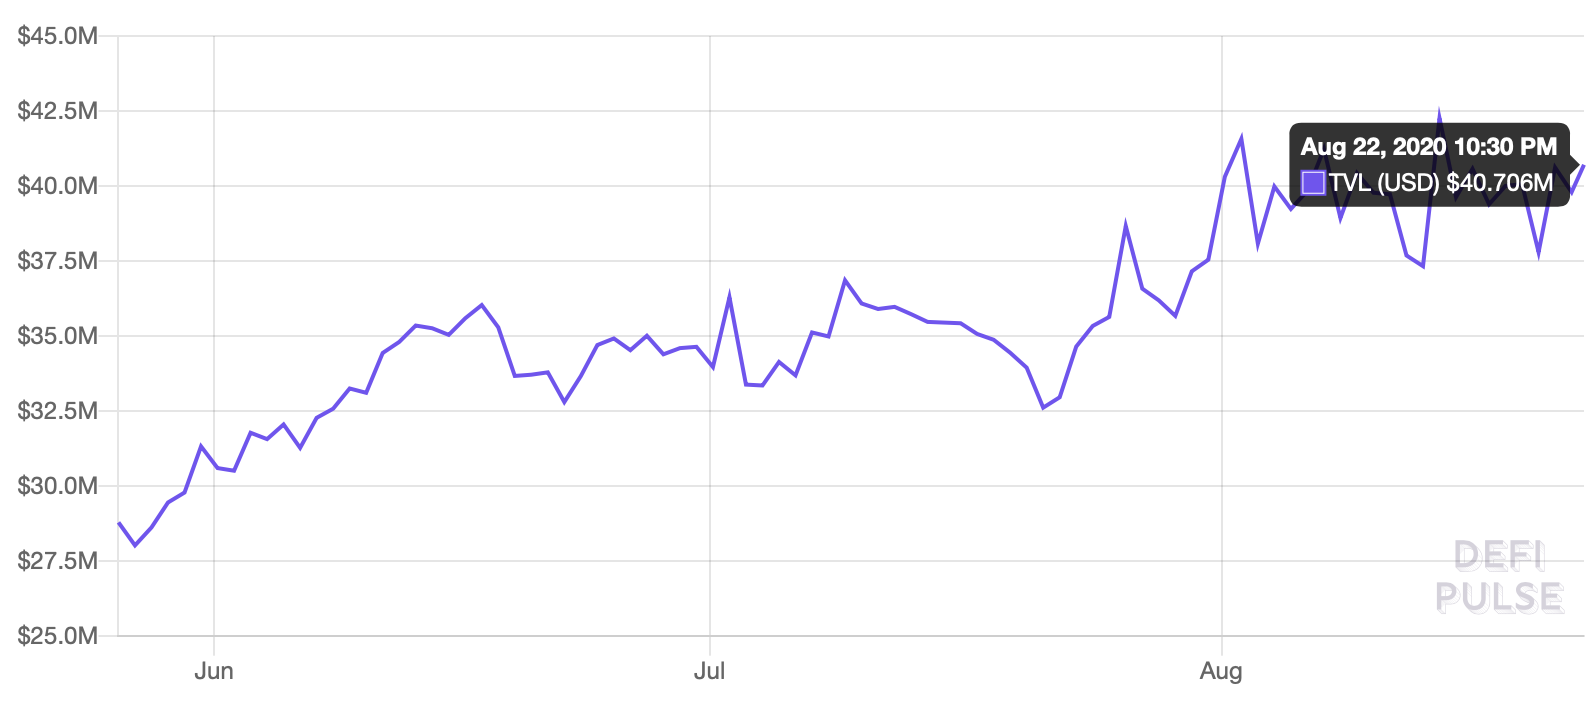
\includegraphics[width=\textwidth]{figures/dydx.png}
%     \caption{Total value locked (USD) in dydx \cite{dydx-cap}. Currently more than 40 M\$}
%     \label{fig:TVL-ACO}
% \end{figure}
% \begin{figure}
%     \centering
%     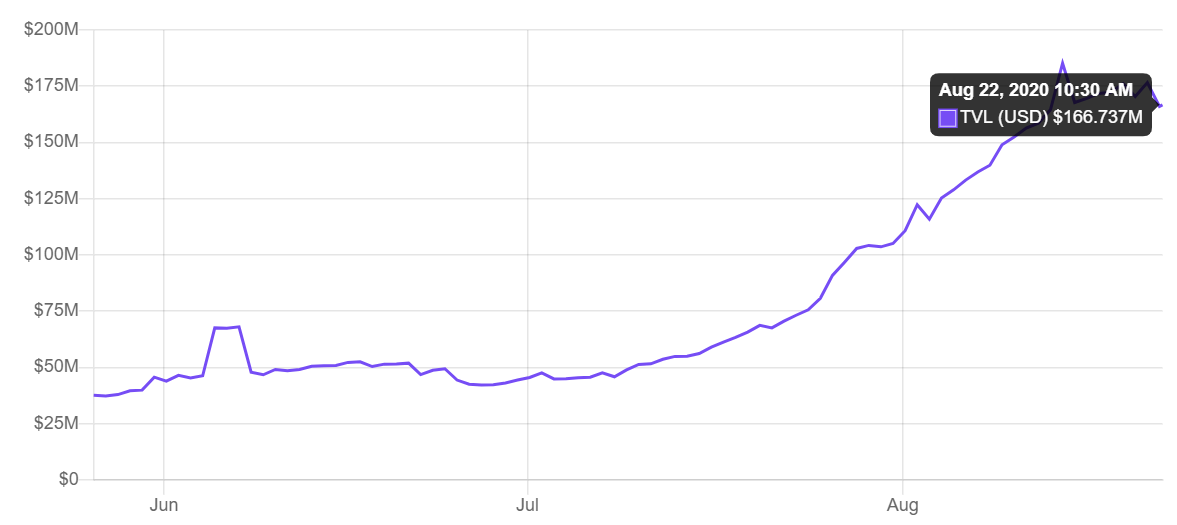
\includegraphics[width=\textwidth]{figures/TVL(USD)-uniswap-90.png}
%     \caption{total value locked (USD) in Uniswap \cite{uniswap-cap}. Currently more than 166 M\$}
%     \label{fig:TVL-Uniswap}
% \end{figure}





% \begin{tabular}{||c c c c c c||} 
%  \hline
%  BTC & ETH & DAI & AE & WBTC & USDC \\ [0.5ex] 
%  \hline\hline
%  20709.97 & 19216.02 & 9598.86 & 10226.57 & 209.33 & 3756.75 \\ [1ex] 
%  \hline
% \end{tabular}


 
The rest of this paper is organized as follows. First of all, in section~\ref{sec:abd} after defining the required terminology and presenting the other preliminaries of our work, we introduce the first \newfateme{model} of atomic bonded debt \newfateme{and discuss about the crucial requirements of an atomic bond service.} Later in section~\ref{sec:abcd}, we redesign our model to build the first practical \emph{atomic bonded cross-chain debt} (ABCD) primitive, \newfateme{and finally by adding additional features to it, we improve its stability across different market behaviours.}


% by using it afterwards, we build the \new{\emph{atomic bonded cross-chain debt} primitive (ABCD)}. 
% first practical version of ABCD component. Finally in the section~\ref{sub:seq-bond} we modify the ABCD to be used in the scenario of cross chain usecase.
% In Section~\ref{sec:relatedWorks}, we review some of the most important and recent studies on traffic classification with details. In Section~\ref{sec:Background}, we present the essential background on machine learning used in proposed methods, including deep learning and decision tree. In Section~\ref{sec:dataset}, we discuss the process of dataset collection and its various aspects, \eg, the reason for using two different datasets. Section~\ref{sec:Methodology} presents our proposed iterative procedure and the details of employed classifiers. The results of our experiments on the gathered data are elaborated in Section~\ref{sec:results}. Finally, we conclude the paper in Section~\ref{sec:conc}, briefing what we have learned throughout this study and how to improve it further.




% \section{Atomic Bonded Debt}
% \label{sec:abd}
% \begin{figure}[h]
%   \centering
%   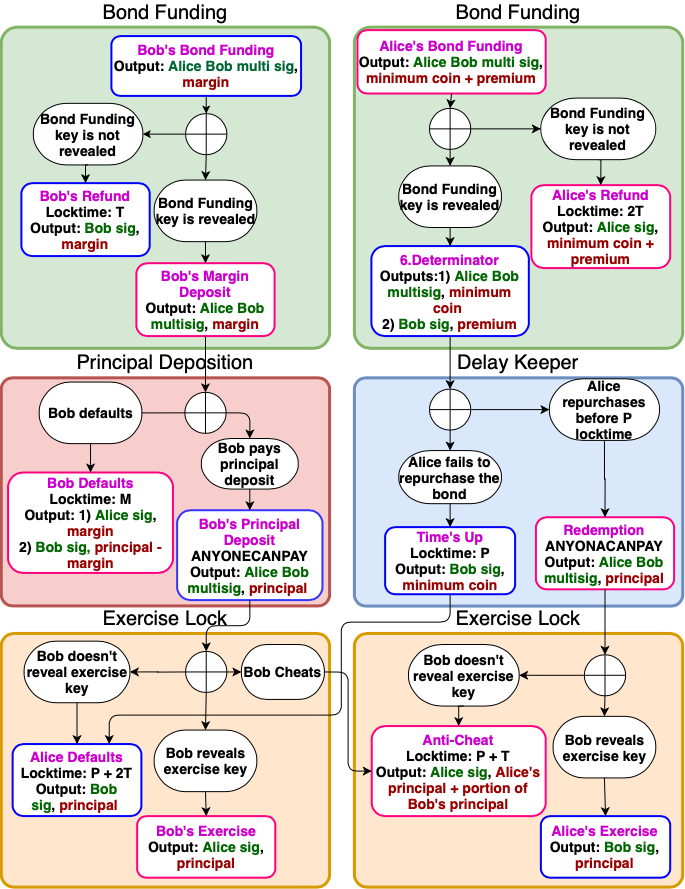
\includegraphics[width=\linewidth]{figures/bond-first.png}
%   \Description{An atomic bonded debt using locktimes}
%   \label{fig:non-collat-bond-no-checkseq}
% \end{figure}
\section{General Overview of Atomic Bonded Debt}
\label{sec:abd}

The idea behind \newfateme{ABCD} is inspired by flash swaps. In a flash swap, the loan is not paid to the borrower unless she pays it back immediately at the same block as borrowed \new{\cite{flashswaps}}. In \abcd this is extended to several blocks i.e. the issuer can \new{repurchase} the bond in more than one block but it contains a secret and the bondholder's signature is required everywhere the capital is being utilized. 

Unsecured bonds or debentures are not backed by some type of collateral. Since this bond is unsecured, the issuer does not have to deposit any margin, unlike the approach used in \new{\cite{liu2018atomic}}. Assume Alice is the issuer and Bob is the purchaser of the bond. She needs to take the capital, exploit it in other contracts, and then \new{repurchase the bond from} Bob with some interest. She also needs Bob to deposit shortly after their contract has been started.

% \subsection{Time Lock based \abcd}
% \label{sub:time-bond}
\newfateme{In this section, we are going to introduce the main challenges for having an atomic bond service. To do so, we designed a general overview of an atomic bond service shown in Fig.}~\ref{fig:non-collat-bond-no-checkseq}. In this , for each transaction, signatures, output amounts, and locktimes are specified. Transactions' border colors show the party who broadcasts the transaction. \newfateme{For now, we assume that all amounts are of the same coin.}
% In this type of bonds, all amounts have to be from the same coin. The cross-chain version of it is discussed later in the section~\ref{sec:abcd}.

\begin{figure}[h]
  \centering
  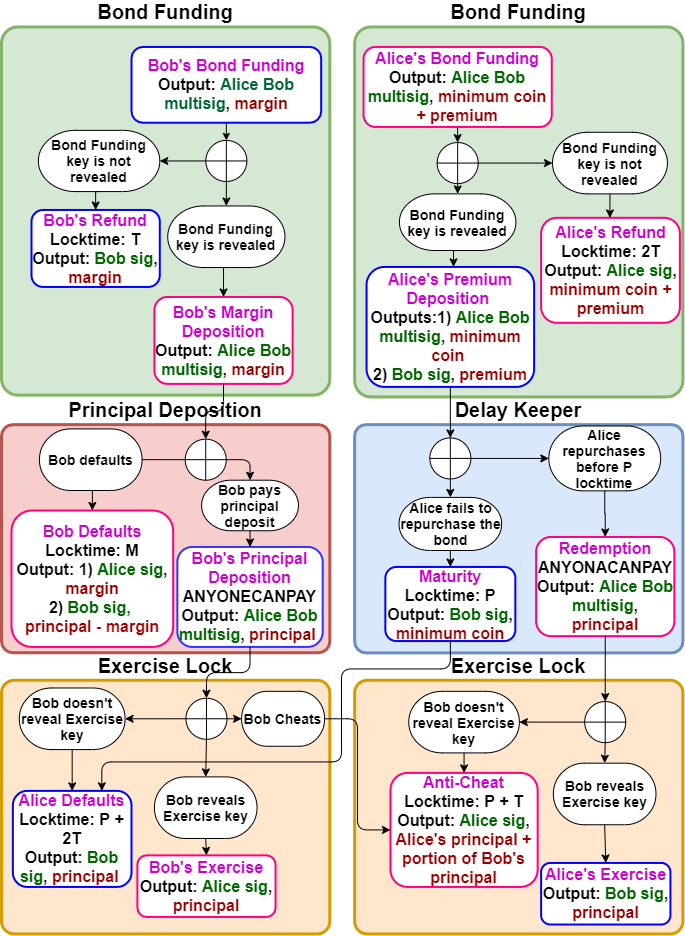
\includegraphics[width=\linewidth]{figures/ABDfateme.png}
  \caption{The general overview of an atomic bond service. Each transaction is shown as a rectangle. On each transaction, signatures, output amount, and locktimes are specified. All outputs are in the same coin. Pink-bordered transactions are broadcast by Alice and blue-bordered ones by Bob. For locktimes, Unix timestamp is used. Upper transactions are broadcast earlier than the lower ones. If there is a line between two transactions, then the source transaction is considered to be an input of the destination transaction.}
  \Description{An atomic bonded debt using locktimes}
  \label{fig:non-collat-bond-no-checkseq}
\end{figure}

Here\newfateme{,} we employ HTLCs to make decisions. If the holder of a secret reveals it before the corresponding timelock deadline, the swap takes place. Otherwise, if she lets the locktime expire, the swap is reverted and all the locked values are given back to their initial owners. The secrets used in \newfateme{this model} are the {\it \Aone} key that the issuer uses to sell and the {\it \keyone} key that the bondholder uses to exercise the bond. In this \newfateme{model}, we use the Unix timestamp as the locktime parameter. We represent the minimum time needed for a mined transaction to be confirmed as $T$. In Bitcoin, it is the time needed to have six subsequent blocks mined which is approximately one hour.

%  Depending on application the bond is being used for, other stages mentioned in the \cite{ourselves} can be appended at the end of the bond structure. The blue box, named as {\it Trust Box} in \cite{ourself} can also be used when the bond is exploited in other contracts such as swaptions \cite{liu2018atomic}, \cite{ourself} i.e. transactions in this boxes may need to be signed by more parties.  Of course in use-cases where additional stages are added, other keys mentioned in \cite{ourself} such as \Atwo key and \Delegation key will be used.

Next\newfateme{,} we explain in detail the process of exercising \newfateme{an atomic bond protocol} which is basically made up of transactions shown in Fig\new{.}~\ref{fig:non-collat-bond-no-checkseq}. First of all, all the transactions are signed and exchanged between the two parties except the bond funding transactions. In this phase, both parties make sure that there is no way the other party cheats on them, since either it is technically impossible or they get punished in case of cheating. This approach is similar to the procedure used by Poon~\etal in the lightening payment channels \new{\cite{poon2016bitcoin}}. After that, by broadcasting each of the transactions in the proper time, the process goes on. The procedure is divided into four different stages. Depending on the application the bond is being used for, other stages can be appended to the procedure and transactions might need to be signed by more parties. However, here we explain the basic structure of the bond itself: 
\begin{itemize}
    \item \textbf{Bond Funding}: 
    The funding transaction for Alice consists of 
    \begin{itemize}
        \item a premium, 
        \item and a very tiny amount for further usage (the minimum acceptable amount of output to be mined by the network miners, for example 546 Satoshis in Bitcoin network at the time of writing).
        % \footnote{In the time we are writing this paper, minimum amount of output in Bitcoin network to be mined by miners is 546 Satoshis}.
    \end{itemize}
    For Bob, the bond funding transaction only contains the margin. Alice has a relatively small amount of time to reveal the \Aone  key to sell the bond. If she issues the bond, the premium goes to Bob and his margin goes to the Bob's margin deposition transaction.
    
    \item \textbf{Principal Deposition}: 
    After selling the bond, each party has to deposit their principal within a specified time interval: Bob $M$ locktime and Alice $P$ ($P > M$). The \emph{\new{Bob's principal} \new{deposition}} and \new{the} \new{\emph{redemption}} transactions have sighash type of anyone-can-pay\footnote{The op-code ANYONECANPAY} since nobody knows all of \newfateme{their} inputs in the first place. Bob can act either ways of:
    \begin{itemize}
        \item If Bob defaults, then Alice takes his margin by broadcasting the \new{\emph{Bob defaults}} transaction. Additionally, she will not fulfill the \newfateme{redemption} transaction. Therefore, Bob can broadcast the \new{\emph{maturity}} transaction, taking the minimum amount of coins which is too small to consider.
        \item If Bob deposits the principal, the bond goes to the \emph{delay keeper} stage.
    \end{itemize}
    The \emph{premium deposition} transaction and the minimum amount of coins are needed so that using this transaction we can force a deadline on Alice depositing her payback by utilizing the locktime on the \new{maturity} transaction. Also, in the case that Alice \new{repurchases} the bond, Bob can not claim that she did not broadcast the \new{redemption} transaction.
    
    \item \textbf{Delay Keeper}: At this stage, Alice has time before a $P$ locktime expires ($P > M$) to fulfill her \new{redemption} transaction. If she does not deposit, Bob will broadcast the \new{maturity} transaction that prevents Alice from fulfilling her \new{redemption} transaction. 
    % Without the presence of the premium deposition transaction, we had no other way to set locktime on the time's up transaction.
    
    \item \textbf{Exercise Lock}: The bond enters this stage when Bob deposits his principal. There are three possible scenarios in here:
    \begin{itemize}
        \item In the last stage, Bob deposited his principal but Alice did not and the \new{maturity} transaction is broadcast. Now Bob does not reveal \keyone key, and using the \new{\emph{Alice defaults}} transaction he takes his principal back.
        
        \item Bob has deposited his principal and Alice has fulfilled her \new{redemption} transaction but Bob avoids revealing the \keyone key. Subsequently, Alice can broadcast the \new{\emph{anti-cheat}} transaction which sends her principal and an amount of punishment from Bob's principal to her. 
        
        \item Both have deposited their principals. Bob reveals \keyone key and they go to the next stage if there is any\footnote{In real-world applications there are usually more stages, since the bond is being used along with other contracts, otherwise it is useless giving ACoins and getting the same ACoins. An example of ABCD implementation along with atomic swap is provided in \cite{abcd-ref}.} and if not, each takes their coins and the procedure ends.
    \end{itemize}

    Note that if Bob delays in broadcasting the \new{maturity} transaction, Alice may broadcast the \new{redemption} and anti-cheat transactions at the very last minute and cheat on Bob.
    
   
\end{itemize}

 \newfateme{The previously presented overview of the atomic bond is well analyzed and seems to be practical. However, there are some problems with its implementation not yet addressed. In every blockchain, signing and spending transactions have a different set of rules,} \new{\eg} \newfateme{in Bitcoin the child transaction has to sign the hash of its parent transaction besides the redeem script. The Bitcoin network considers the inputs of a transaction when calculating its hash. To be able to create a transaction that spends a transaction's output, we need to calculate the parent transaction's hash correctly. Therefore, all of a transaction's inputs have to be determined, before creating its output spender. Hence, the transactions in the exercise lock sections are impossible to be signed at the beginning of the protocol. In the subsequent pages, we will prepare our primitives to overcome this issue.}


\section{Atomic Bonded Cross-chain Debt}
\label{sec:abcd}

Since the Alice's time's up transaction in the ABD primitive needs to be shared in both Alice's and Bob's stages, this form of bond can not be used across different blockchains. To solve the problem of interoperability for the atomic bond we have redesigned our model using check-sequence-verify\footnote{The up-code CHECKSEQVERIFY}. In this section, we first build an intermediary component that has the same functionality as ABD. After that, we introduce the ABCD that can be actually used between different blockchains.
% At the time of writing, there are more than a thousand implemented blockchains working. One of our concerns about the non-collateralized bond component is the possibility of using checkseqverify. If a blockchain does not support this type of opcode we can not use this type of bond in it.
Using the check-sequence-verify, the minimum amount of coins for the determinator transaction and the delay keeper stage are removed from the component.
% Using the "check sequence verify" there is no need for delay keeper stage and temp transaction and the minimum amount of coins used in the previous type.
\begin{figure}[h]
  \centering
  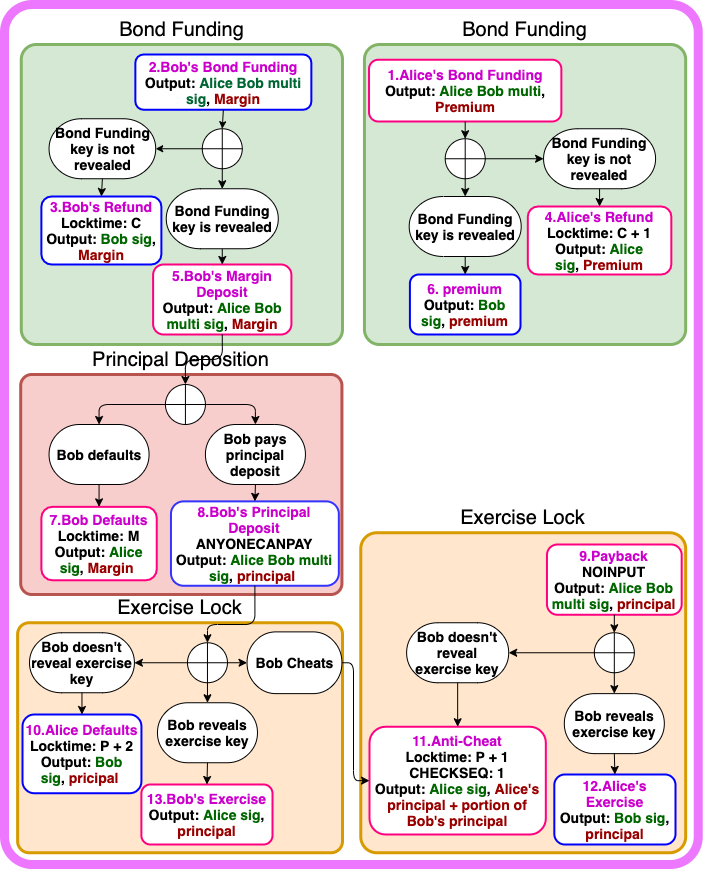
\includegraphics[width=\linewidth]{figures/bond-second.png}
  \caption{The ABD component using checkseq. On each transaction, signatures, output amount and locktimes are specified. All outputs are in the same coin. Pink-bordered transactions are broadcast by Alice and blue-bordered ones by Bob. For locktimes, block height is used. Upper transactions are broadcast earlier than the lower ones. If there is a line between two transactions, then the source transaction is considered to be an input of the destination transaction.}
  \Description{An atomic bonded debt using checkseqverify}
  \label{fig:non-collat-bond}
\end{figure}

The intermediary ABD component is demonstrated in Fig~\ref{fig:non-collat-bond}. To present this type of ABD we use block height as the locktime parameter, however the Unix timestamp can also be used. The procedure is discussed below:

\begin{itemize}
    \item \textbf{Bond Funding}: Alice's funding includes premium and Bob's includes margin.
    
    \item \textbf{Principal Deposition}: 
        After issuing the bond, similar to the original ABD, each party has to deposit his principal within a specified time interval: Bob $M$ locktime and Alice $P$ ($P > M$). Bob's principal deposit transaction has sighash type of anyone-can-pay but Alice's has "no-input" type since one of Bob's inputs is determined while none of Alice's inputs is clear at the time of creating the transaction. Bob can behave in one of the two following ways:
    \begin{itemize}
        \item He defaults, then Alice takes his margin by broadcasting the Bob defaults transaction.
        \item He deposits the principal, then the procedure goes to the next stage.
    \end{itemize}
    
    \item \textbf{Exercise Lock}: If Bob deposits his principal before the locktime, Alice has time before a $P$ locktime expires to pay her debt back. As mentioned earlier, the payback transaction has sighash type of no-input. The "checkseq 1" in the anti-cheat transaction, forces this transaction to have a minimum block distance of 1 from its parent i.e. the anti-cheat transaction can only be mined in a block with a higher block height than the block which Alice's payback transaction is in, hence Bob has enough time to reveal the \keyone key. Note that the 1 block height difference may have to vary in different blockchains. For example in bitcoin, the minimum block height needed to elapse for the transactions to be confirmed is 6 blocks. Thus, we have to use "checkseq 6" in bitcoin. However, in this context, we assume the general case of 1 block.
    
    After Bob's principal deposition, there are two possible scenarios: 
    \begin{itemize}
        \item Alice succeeds to payback. Bob reveals the \keyone key. The result is similar to the original ABD. 
        
        \item Alice does not broadcast the payback transaction hence Bob avoids exposing the \keyone key and his principal is sent back to himself. To achieve this, Bob gives Alice $P + 2$ locktime to convince him to reveal the \keyone key and if this deadline is passed, he will broadcast the Alice defaults transaction which gives him back his principal.
        
        \item Alice fulfills her payback transaction but Bob does not reveal the \keyone key. In this case, Alice can broadcast the anti-cheat transaction to get her principal and a portion of Bob's principal as the punishment. Note that, since the anti-cheat transaction has a locktime of $P + 1$ and a checkseq of 1 and the Alice's defaults transaction has a locktime of $P + 1$, Alice has to broadcast her payback before $P$. Otherwise, she would not have enough time to broadcast the anti-cheat transaction in the case of Bob cheating. In other words, if the Alice's payback transaction is mined in a block of at least $P + 1$ height and Bob does not reveal \keyone key, she can not get the anti-cheat transaction mined before block $P + 2$. Therefore, Bob can broadcast the Alice defaults in the $P + 1$th block and avoid giving her the capital.
    \end{itemize}
\end{itemize}

The reason which prevents the intermediary ABD component to be used in a cross-chain environment is that
% The above form still can not be used for parties on the different blockchains, since 
the anti-cheat transaction has inputs from both Alice's and Bob's sides. To overcome this issue, before exploiting any bond contract, Bob, which is considered to be an exchange or somebody who has a reasonable amount of assets in different blockchains, can deposit some assets as a bond guarantee in any desired chain. This way, Bob can offer his customers a cross-chain bond service that accepts his payback in the other chain. This modification can be seen in Fig.\ref{fig:cross-chain-non-collat-bond}. In \abcd, we use Unix timestamp for locktimes and we consider the maximum time among all of involved blockchains since in different blockchains the number of blocks needed for confirmation is different.


\begin{figure}[]
  \centering
  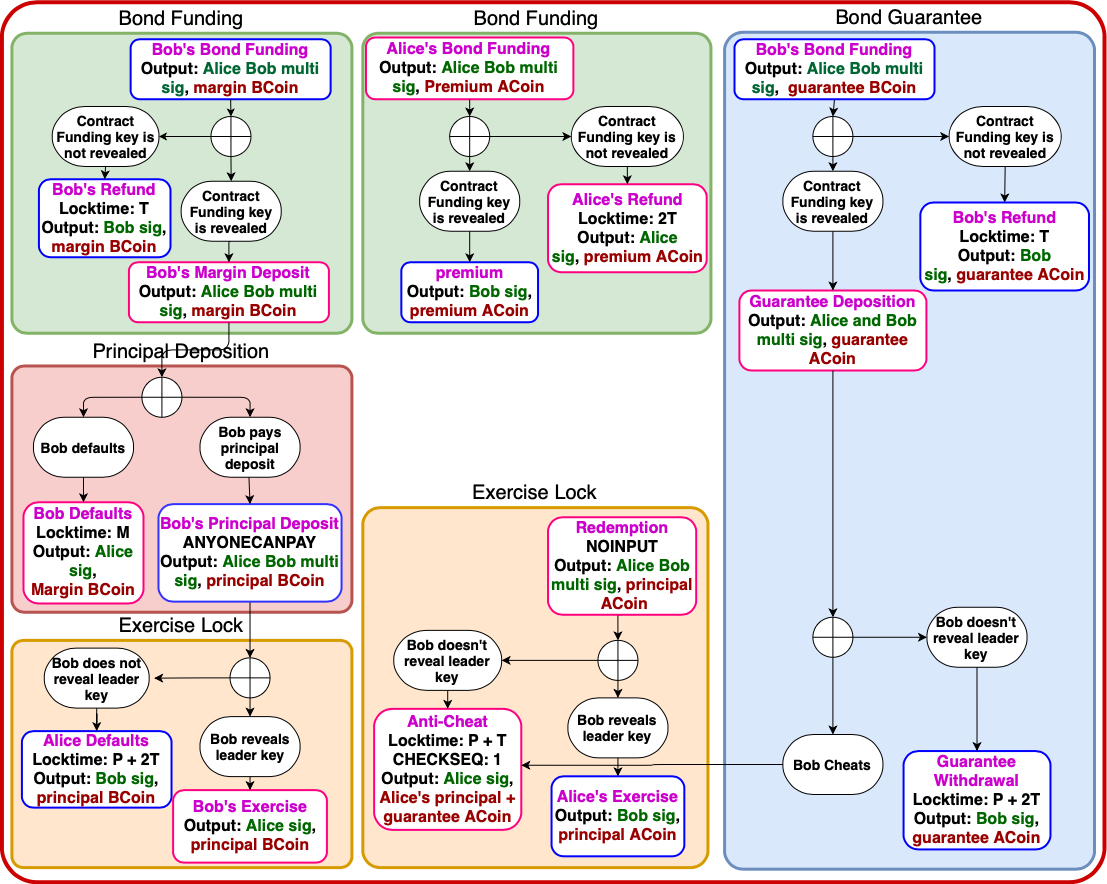
\includegraphics[width=\linewidth]{figures/bond-third.png}
  \caption{The ABCD across different chains. On each transaction, signatures, output amount and locktimes are specified. Bob's depositions are in Bcoin and Alice's in Acoin. Pink-bordered transactions are broadcast by Alice and blue-bordered ones by Bob. For checkseq, block height is used. For locktimes, Unix timestamp is used. Upper transactions are broadcast earlier than the lower ones. If there is a line between two transaction, then the source transactions is considered to be an input of the destination transaction.}
  \Description{A cross-chain atomic bonded debt.}
  \label{fig:cross-chain-non-collat-bond}
\end{figure}

The difference between the intermediary ABD component and the ABCD primitive is addition of the guarantee withdrawal transaction. Whether Alice defaults or the bond is successfully executed, Bob has to broadcast the guarantee withdrawal transaction. Other parts are the same in both procedures.
% The details of the ABCD is same as the intermediary ABD except for 

\section{Conslusion}

In this paper, we first introduced ABD which is a single-chain bond contract. \new{Afterward,} by extending its design, we derived ABCD to achieve the goal of providing an interoperable cross-chain bond. Collectively, we have employed the well-known atomic cross-chain swaps for building ABCD as a primitive for uncollateralized DeFi. Potential use cases include but are not limited to exploiting arbitrage opportunities between swaptions without owning any capital or any other similar use case of flash loans and flash swaps with two major improvements: 
\begin{itemize}
    \item Despite the similarities, instead of being a ``flash'' loan which must be repaid within a block, \abcd can span an arbitrary long period of time for the issuer to trade or invest with the capital before the bond reaches maturity. The significance of this feature is highlighted by noting that this is not possible even in conventional financial systems to have an unsecured debt without a credit system. More precisely, this property is only possible due to full transparency and traceability of cryptocurrencies.
    \item Our proposed bond primitive does not require a Turing-complete programming language and bitcoin scripting language is sufficient to implement our method which is completely based on HTLC. While most DeFi protocols rely heavily on smart contracts or third parties which make them susceptible to security issues, \abcd can be flexibly used on the wide variety of HTLC-compatible blockchains and in particular, supports bitcoin natively.
\end{itemize}
 
\section{Future Work}

As mentioned earlier, \abcd can be used along with other primitives in order to form more complex contracts. Depending on the application-specific domain, the current structure of \abcd might be either sufficient or not. In a future work, we aim to customize this structure to be fully compatible for integration in more complex systems.

On the other hand, there exist many variations of HTLC which in turn imply different categories of atomic swaps with different properties. The modular structure of our design enables similar variations on ABCD with the associated properties which can be explored in a future work.  

% \section{Introduction}
% ACM's consolidated article template, introduced in 2017, provides a
% consistent \LaTeX\ style for use across ACM publications, and
% incorporates accessibility and metadata-extraction functionality
% necessary for future Digital Library endeavors. Numerous ACM and
% SIG-specific \LaTeX\ templates have been examined, and their unique
% features incorporated into this single new template.

% If you are new to publishing with ACM, this document is a valuable
% guide to the process of preparing your work for publication. If you
% have published with ACM before, this document provides insight and
% instruction into more recent changes to the article template.

% The ``\verb|acmart|'' document class can be used to prepare articles
% for any ACM publication --- conference or journal, and for any stage
% of publication, from review to final ``camera-ready'' copy, to the
% author's own version, with {\itshape very} few changes to the source.

% \section{Template Overview}
% As noted in the introduction, the ``\verb|acmart|'' document class can
% be used to prepare many different kinds of documentation --- a
% double-blind initial submission of a full-length technical paper, a
% two-page SIGGRAPH Emerging Technologies abstract, a ``camera-ready''
% journal article, a SIGCHI Extended Abstract, and more --- all by
% selecting the appropriate {\itshape template style} and {\itshape
%   template parameters}.

% This document will explain the major features of the document
% class. For further information, the {\itshape \LaTeX\ User's Guide} is
% available from
% \url{https://www.acm.org/publications/proceedings-template}.

% \subsection{Template Styles}

% The primary parameter given to the ``\verb|acmart|'' document class is
% the {\itshape template style} which corresponds to the kind of publication
% or SIG publishing the work. This parameter is enclosed in square
% brackets and is a part of the {\verb|documentclass|} command:
% \begin{verbatim}
%   \documentclass[STYLE]{acmart}
% \end{verbatim}

% Journals use one of three template styles. All but three ACM journals
% use the {\verb|acmsmall|} template style:
% \begin{itemize}
% \item {\verb|acmsmall|}: The default journal template style.
% \item {\verb|acmlarge|}: Used by JOCCH and TAP.
% \item {\verb|acmtog|}: Used by TOG.
% \end{itemize}

% The majority of conference proceedings documentation will use the {\verb|acmconf|} template style.
% \begin{itemize}
% \item {\verb|acmconf|}: The default proceedings template style.
% \item{\verb|sigchi|}: Used for SIGCHI conference articles.
% \item{\verb|sigchi-a|}: Used for SIGCHI ``Extended Abstract'' articles.
% \item{\verb|sigplan|}: Used for SIGPLAN conference articles.
% \end{itemize}

% \subsection{Template Parameters}

% In addition to specifying the {\itshape template style} to be used in
% formatting your work, there are a number of {\itshape template parameters}
% which modify some part of the applied template style. A complete list
% of these parameters can be found in the {\itshape \LaTeX\ User's Guide.}

% Frequently-used parameters, or combinations of parameters, include:
% \begin{itemize}
% \item {\verb|anonymous,review|}: Suitable for a ``double-blind''
%   conference submission. Anonymizes the work and includes line
%   numbers. Use with the \verb|\acmSubmissionID| command to print the
%   submission's unique ID on each page of the work.
% \item{\verb|authorversion|}: Produces a version of the work suitable
%   for posting by the author.
% \item{\verb|screen|}: Produces colored hyperlinks.
% \end{itemize}

% This document uses the following string as the first command in the
% source file:
% \begin{verbatim}
% \documentclass[sigconf]{acmart}
% \end{verbatim}

% \section{Modifications}

% Modifying the template --- including but not limited to: adjusting
% margins, typeface sizes, line spacing, paragraph and list definitions,
% and the use of the \verb|\vspace| command to manually adjust the
% vertical spacing between elements of your work --- is not allowed.

% {\bfseries Your document will be returned to you for revision if
%   modifications are discovered.}

% \section{Typefaces}

% The ``\verb|acmart|'' document class requires the use of the
% ``Libertine'' typeface family. Your \TeX\ installation should include
% this set of packages. Please do not substitute other typefaces. The
% ``\verb|lmodern|'' and ``\verb|ltimes|'' packages should not be used,
% as they will override the built-in typeface families.

% \section{Title Information}

% The title of your work should use capital letters appropriately -
% \url{https://capitalizemytitle.com/} has useful rules for
% capitalization. Use the {\verb|title|} command to define the title of
% your work. If your work has a subtitle, define it with the
% {\verb|subtitle|} command.  Do not insert line breaks in your title.

% If your title is lengthy, you must define a short version to be used
% in the page headers, to prevent overlapping text. The \verb|title|
% command has a ``short title'' parameter:
% \begin{verbatim}
%   \title[short title]{full title}
% \end{verbatim}

% \section{Authors and Affiliations}

% Each author must be defined separately for accurate metadata
% identification. Multiple authors may share one affiliation. Authors'
% names should not be abbreviated; use full first names wherever
% possible. Include authors' e-mail addresses whenever possible.

% Grouping authors' names or e-mail addresses, or providing an ``e-mail
% alias,'' as shown below, is not acceptable:
% \begin{verbatim}
%   \author{Brooke Aster, David Mehldau}
%   \email{dave,judy,steve@university.edu}
%   \email{firstname.lastname@phillips.org}
% \end{verbatim}

% The \verb|authornote| and \verb|authornotemark| commands allow a note
% to apply to multiple authors --- for example, if the first two authors
% of an article contributed equally to the work.

% If your author list is lengthy, you must define a shortened version of
% the list of authors to be used in the page headers, to prevent
% overlapping text. The following command should be placed just after
% the last \verb|\author{}| definition:
% \begin{verbatim}
%   \renewcommand{\shortauthors}{McCartney, et al.}
% \end{verbatim}
% Omitting this command will force the use of a concatenated list of all
% of the authors' names, which may result in overlapping text in the
% page headers.

% The article template's documentation, available at
% \url{https://www.acm.org/publications/proceedings-template}, has a
% complete explanation of these commands and tips for their effective
% use.

% Note that authors' addresses are mandatory for journal articles.

% \section{Rights Information}

% Authors of any work published by ACM will need to complete a rights
% form. Depending on the kind of work, and the rights management choice
% made by the author, this may be copyright transfer, permission,
% license, or an OA (open access) agreement.

% Regardless of the rights management choice, the author will receive a
% copy of the completed rights form once it has been submitted. This
% form contains \LaTeX\ commands that must be copied into the source
% document. When the document source is compiled, these commands and
% their parameters add formatted text to several areas of the final
% document:
% \begin{itemize}
% \item the ``ACM Reference Format'' text on the first page.
% \item the ``rights management'' text on the first page.
% \item the conference information in the page header(s).
% \end{itemize}

% Rights information is unique to the work; if you are preparing several
% works for an event, make sure to use the correct set of commands with
% each of the works.

% The ACM Reference Format text is required for all articles over one
% page in length, and is optional for one-page articles (abstracts).

% \section{CCS Concepts and User-Defined Keywords}

% Two elements of the ``acmart'' document class provide powerful
% taxonomic tools for you to help readers find your work in an online
% search.

% The ACM Computing Classification System ---
% \url{https://www.acm.org/publications/class-2012} --- is a set of
% classifiers and concepts that describe the computing
% discipline. Authors can select entries from this classification
% system, via \url{https://dl.acm.org/ccs/ccs.cfm}, and generate the
% commands to be included in the \LaTeX\ source.

% User-defined keywords are a comma-separated list of words and phrases
% of the authors' choosing, providing a more flexible way of describing
% the research being presented.

% CCS concepts and user-defined keywords are required for for all
% articles over two pages in length, and are optional for one- and
% two-page articles (or abstracts).

% \section{Sectioning Commands}

% Your work should use standard \LaTeX\ sectioning commands:
% \verb|section|, \verb|subsection|, \verb|subsubsection|, and
% \verb|paragraph|. They should be numbered; do not remove the numbering
% from the commands.

% Simulating a sectioning command by setting the first word or words of
% a paragraph in boldface or italicized text is {\bfseries not allowed.}

% \section{Tables}

% The ``\verb|acmart|'' document class includes the ``\verb|booktabs|''
% package --- \url{https://ctan.org/pkg/booktabs} --- for preparing
% high-quality tables.

% Table captions are placed {\itshape above} the table.

% Because tables cannot be split across pages, the best placement for
% them is typically the top of the page nearest their initial cite.  To
% ensure this proper ``floating'' placement of tables, use the
% environment \textbf{table} to enclose the table's contents and the
% table caption.  The contents of the table itself must go in the
% \textbf{tabular} environment, to be aligned properly in rows and
% columns, with the desired horizontal and vertical rules.  Again,
% detailed instructions on \textbf{tabular} material are found in the
% \textit{\LaTeX\ User's Guide}.

% Immediately following this sentence is the point at which
% Table~\ref{tab:freq} is included in the input file; compare the
% placement of the table here with the table in the printed output of
% this document.

% \begin{table}
%   \caption{Frequency of Special Characters}
%   \label{tab:freq}
%   \begin{tabular}{ccl}
%     \toprule
%     Non-English or Math&Frequency&Comments\\
%     \midrule
%     \O & 1 in 1,000& For Swedish names\\
%     $\pi$ & 1 in 5& Common in math\\
%     \$ & 4 in 5 & Used in business\\
%     $\Psi^2_1$ & 1 in 40,000& Unexplained usage\\
%   \bottomrule
% \end{tabular}
% \end{table}

% To set a wider table, which takes up the whole width of the page's
% live area, use the environment \textbf{table*} to enclose the table's
% contents and the table caption.  As with a single-column table, this
% wide table will ``float'' to a location deemed more
% desirable. Immediately following this sentence is the point at which
% Table~\ref{tab:commands} is included in the input file; again, it is
% instructive to compare the placement of the table here with the table
% in the printed output of this document.

% \begin{table*}
%   \caption{Some Typical Commands}
%   \label{tab:commands}
%   \begin{tabular}{ccl}
%     \toprule
%     Command &A Number & Comments\\
%     \midrule
%     \texttt{{\char'134}author} & 100& Author \\
%     \texttt{{\char'134}table}& 300 & For tables\\
%     \texttt{{\char'134}table*}& 400& For wider tables\\
%     \bottomrule
%   \end{tabular}
% \end{table*}

% Always use midrule to separate table header rows from data rows, and
% use it only for this purpose. This enables assistive technologies to
% recognise table headers and support their users in navigating tables
% more easily.

% \section{Math Equations}
% You may want to display math equations in three distinct styles:
% inline, numbered or non-numbered display.  Each of the three are
% discussed in the next sections.

% \subsection{Inline (In-text) Equations}
% A formula that appears in the running text is called an inline or
% in-text formula.  It is produced by the \textbf{math} environment,
% which can be invoked with the usual
% \texttt{{\char'134}begin\,\ldots{\char'134}end} construction or with
% the short form \texttt{\$\,\ldots\$}. You can use any of the symbols
% and structures, from $\alpha$ to $\omega$, available in
% \LaTeX~\cite{Lamport:LaTeX}; this section will simply show a few
% examples of in-text equations in context. Notice how this equation:
% \begin{math}
%   \lim_{n\rightarrow \infty}x=0
% \end{math},
% set here in in-line math style, looks slightly different when
% set in display style.  (See next section).

% \subsection{Display Equations}
% A numbered display equation---one set off by vertical space from the
% text and centered horizontally---is produced by the \textbf{equation}
% environment. An unnumbered display equation is produced by the
% \textbf{displaymath} environment.

% Again, in either environment, you can use any of the symbols and
% structures available in \LaTeX\@; this section will just give a couple
% of examples of display equations in context.  First, consider the
% equation, shown as an inline equation above:
% \begin{equation}
%   \lim_{n\rightarrow \infty}x=0
% \end{equation}
% Notice how it is formatted somewhat differently in
% the \textbf{displaymath}
% environment.  Now, we'll enter an unnumbered equation:
% \begin{displaymath}
%   \sum_{i=0}^{\infty} x + 1
% \end{displaymath}
% and follow it with another numbered equation:
% \begin{equation}
%   \sum_{i=0}^{\infty}x_i=\int_{0}^{\pi+2} f
% \end{equation}
% just to demonstrate \LaTeX's able handling of numbering.

% \section{Figures}

% The ``\verb|figure|'' environment should be used for figures. One or
% more images can be placed within a figure. If your figure contains
% third-party material, you must clearly identify it as such, as shown
% in the example below.
% \begin{figure}[h]
%   \centering
%   \includegraphics[width=\linewidth]{sample-franklin}
%   \caption{1907 Franklin Model D roadster. Photograph by Harris \&
%     Ewing, Inc. [Public domain], via Wikimedia
%     Commons. (\url{https://goo.gl/VLCRBB}).}
%   \Description{A woman and a girl in white dresses sit in an open car.}
% \end{figure}

% Your figures should contain a caption which describes the figure to
% the reader.

% Figure captions are placed {\itshape below} the figure.

% Every figure should also have a figure description unless it is purely
% decorative. These descriptions convey what’s in the image to someone
% who cannot see it. They are also used by search engine crawlers for
% indexing images, and when images cannot be loaded.

% A figure description must be unformatted plain text less than 2000
% characters long (including spaces).  {\bfseries Figure descriptions
%   should not repeat the figure caption – their purpose is to capture
%   important information that is not already provided in the caption or
%   the main text of the paper.} For figures that convey important and
% complex new information, a short text description may not be
% adequate. More complex alternative descriptions can be placed in an
% appendix and referenced in a short figure description. For example,
% provide a data table capturing the information in a bar chart, or a
% structured list representing a graph.  For additional information
% regarding how best to write figure descriptions and why doing this is
% so important, please see
% \url{https://www.acm.org/publications/taps/describing-figures/}.

% \subsection{The ``Teaser Figure''}

% A ``teaser figure'' is an image, or set of images in one figure, that
% are placed after all author and affiliation information, and before
% the body of the article, spanning the page. If you wish to have such a
% figure in your article, place the command immediately before the
% \verb|\maketitle| command:
% \begin{verbatim}
%   \begin{teaserfigure}
%     \includegraphics[width=\textwidth]{sampleteaser}
%     \caption{figure caption}
%     \Description{figure description}
%   \end{teaserfigure}
% \end{verbatim}

% \section{Citations and Bibliographies}

% The use of \BibTeX\ for the preparation and formatting of one's
% references is strongly recommended. Authors' names should be complete
% --- use full first names (``Donald E. Knuth'') not initials
% (``D. E. Knuth'') --- and the salient identifying features of a
% reference should be included: title, year, volume, number, pages,
% article DOI, etc.

% The bibliography is included in your source document with these two
% commands, placed just before the \verb|\end{document}| command:
% \begin{verbatim}
%   \bibliographystyle{ACM-Reference-Format}
%   \bibliography{bibfile}
% \end{verbatim}
% where ``\verb|bibfile|'' is the name, without the ``\verb|.bib|''
% suffix, of the \BibTeX\ file.

% Citations and references are numbered by default. A small number of
% ACM publications have citations and references formatted in the
% ``author year'' style; for these exceptions, please include this
% command in the {\bfseries preamble} (before the command
% ``\verb|\begin{document}|'') of your \LaTeX\ source:
% \begin{verbatim}
%   \citestyle{acmauthoryear}
% \end{verbatim}

%   Some examples.  A paginated journal article \cite{Abril07}, an
%   enumerated journal article \cite{Cohen07}, a reference to an entire
%   issue \cite{JCohen96}, a monograph (whole book) \cite{Kosiur01}, a
%   monograph/whole book in a series (see 2a in spec. document)
%   \cite{Harel79}, a divisible-book such as an anthology or compilation
%   \cite{Editor00} followed by the same example, however we only output
%   the series if the volume number is given \cite{Editor00a} (so
%   Editor00a's series should NOT be present since it has no vol. no.),
%   a chapter in a divisible book \cite{Spector90}, a chapter in a
%   divisible book in a series \cite{Douglass98}, a multi-volume work as
%   book \cite{Knuth97}, a couple of articles in a proceedings (of a
%   conference, symposium, workshop for example) (paginated proceedings
%   article) \cite{Andler79, Hagerup1993}, a proceedings article with
%   all possible elements \cite{Smith10}, an example of an enumerated
%   proceedings article \cite{VanGundy07}, an informally published work
%   \cite{Harel78}, a couple of preprints \cite{Bornmann2019,
%     AnzarootPBM14}, a doctoral dissertation \cite{Clarkson85}, a
%   master's thesis: \cite{anisi03}, an online document / world wide web
%   resource \cite{Thornburg01, Ablamowicz07, Poker06}, a video game
%   (Case 1) \cite{Obama08} and (Case 2) \cite{Novak03} and \cite{Lee05}
%   and (Case 3) a patent \cite{JoeScientist001}, work accepted for
%   publication \cite{rous08}, 'YYYYb'-test for prolific author
%   \cite{SaeediMEJ10} and \cite{SaeediJETC10}. Other cites might
%   contain 'duplicate' DOI and URLs (some SIAM articles)
%   \cite{Kirschmer:2010:AEI:1958016.1958018}. Boris / Barbara Beeton:
%   multi-volume works as books \cite{MR781536} and \cite{MR781537}. A
%   couple of citations with DOIs:
%   \cite{2004:ITE:1009386.1010128,Kirschmer:2010:AEI:1958016.1958018}. Online
%   citations: \cite{TUGInstmem, Thornburg01, CTANacmart}. Artifacts:
%   \cite{R} and \cite{UMassCitations}.

% \section{Acknowledgments}

% Identification of funding sources and other support, and thanks to
% individuals and groups that assisted in the research and the
% preparation of the work should be included in an acknowledgment
% section, which is placed just before the reference section in your
% document.

% This section has a special environment:
% \begin{verbatim}
%   \begin{acks}
%   ...
%   \end{acks}
% \end{verbatim}
% so that the information contained therein can be more easily collected
% during the article metadata extraction phase, and to ensure
% consistency in the spelling of the section heading.

% Authors should not prepare this section as a numbered or unnumbered {\verb|\section|}; please use the ``{\verb|acks|}'' environment.

% \section{Appendices}

% If your work needs an appendix, add it before the
% ``\verb|\end{document}|'' command at the conclusion of your source
% document.

% Start the appendix with the ``\verb|appendix|'' command:
% \begin{verbatim}
%   \appendix
% \end{verbatim}
% and note that in the appendix, sections are lettered, not
% numbered. This document has two appendices, demonstrating the section
% and subsection identification method.

% \section{SIGCHI Extended Abstracts}

% The ``\verb|sigchi-a|'' template style (available only in \LaTeX\ and
% not in Word) produces a landscape-orientation formatted article, with
% a wide left margin. Three environments are available for use with the
% ``\verb|sigchi-a|'' template style, and produce formatted output in
% the margin:
% \begin{itemize}
% \item {\verb|sidebar|}:  Place formatted text in the margin.
% \item {\verb|marginfigure|}: Place a figure in the margin.
% \item {\verb|margintable|}: Place a table in the margin.
% \end{itemize}

% %%
% %% The acknowledgments section is defined using the "acks" environment
% %% (and NOT an unnumbered section). This ensures the proper
% %% identification of the section in the article metadata, and the
% %% consistent spelling of the heading.
% \begin{acks}
% To Robert, for the bagels and explaining CMYK and color spaces.
% \end{acks}

% %%
% %% The next two lines define the bibliography style to be used, and
% %% the bibliography file.
\bibliographystyle{ACM-Reference-Format}
\bibliography{sections/bibliography.bib}

% %%
% %% If your work has an appendix, this is the place to put it.
% \appendix

% \section{Research Methods}

% \subsection{Part One}

% Lorem ipsum dolor sit amet, consectetur adipiscing elit. Morbi
% malesuada, quam in pulvinar varius, metus nunc fermentum urna, id
% sollicitudin purus odio sit amet enim. Aliquam ullamcorper eu ipsum
% vel mollis. Curabitur quis dictum nisl. Phasellus vel semper risus, et
% lacinia dolor. Integer ultricies commodo sem nec semper.

% \subsection{Part Two}

% Etiam commodo feugiat nisl pulvinar pellentesque. Etiam auctor sodales
% ligula, non varius nibh pulvinar semper. Suspendisse nec lectus non
% ipsum convallis congue hendrerit vitae sapien. Donec at laoreet
% eros. Vivamus non purus placerat, scelerisque diam eu, cursus
% ante. Etiam aliquam tortor auctor efficitur mattis.

% \section{Online Resources}

% Nam id fermentum dui. Suspendisse sagittis tortor a nulla mollis, in
% pulvinar ex pretium. Sed interdum orci quis metus euismod, et sagittis
% enim maximus. Vestibulum gravida massa ut felis suscipit
% congue. Quisque mattis elit a risus ultrices commodo venenatis eget
% dui. Etiam sagittis eleifend elementum.

% Nam interdum magna at lectus dignissim, ac dignissim lorem
% rhoncus. Maecenas eu arcu ac neque placerat aliquam. Nunc pulvinar
% massa et mattis lacinia.

\end{document}
\endinput
%%
%% End of file `sample-sigconf.tex'.
